%-------------------------------------------------------------------
% Document class and package definitions
%-------------------------------------------------------------------
\documentclass[12pt,a4paper,openright,final,twoside,ieeetran]{main}
\definecolor{mGreen}{rgb}{0,0.6,0}
\definecolor{mGray}{rgb}{0.5,0.5,0.5}
\definecolor{mPurple}{rgb}{0.58,0,0.82}
\definecolor{backgroundColour}{rgb}{0.95,0.95,0.92}

\lstdefinestyle{CStyle}{
    backgroundcolor=\color{backgroundColour},   
    commentstyle=\color{mGreen},
    keywordstyle=\color{magenta},
    numberstyle=\tiny\color{mGray},
    stringstyle=\color{mPurple},
    basicstyle=\footnotesize,
    breakatwhitespace=false,         
    breaklines=true,                 
    captionpos=b,                    
    keepspaces=true,                 
    numbers=left,                    
    numbersep=5pt,                  
    showspaces=false,                
    showstringspaces=false,
    showtabs=false,                  
    tabsize=2,
    language=C
}
\lstdefinestyle{SQLStyle}{
    backgroundcolor=\color{backgroundColour},   
    commentstyle=\color{mGreen},
    keywordstyle=\color{magenta},
    numberstyle=\tiny\color{mGray},
    stringstyle=\color{mPurple},
    basicstyle=\footnotesize,
    breakatwhitespace=false,         
    breaklines=true,                 
    captionpos=b,                    
    keepspaces=true,                 
    numbers=left,                    
    numbersep=5pt,                  
    showspaces=false,                
    showstringspaces=false,
    showtabs=false,                  
    tabsize=2,
    language=SQL
}



%Included for Gather Purpose only:
%input "thesisreferences.bib"

\begin{document}
{\parskip=0pt
\defaultbibliography{thesisreferences.bib}     %% Change this only.
\defaultbibliographystyle{unsrt}        %% Could be changed if you like 
                                           %% references typeset differently.
%-------------------------------------------------------------------
% Define title, author, etc.
%-------------------------------------------------------------------
\def\thesistitle{Embedded IoT for Eclipse Arrowhead}
\def\theauthor{Albin Martinsson}
\def\theaddress{Dept.\ of Computer Science and Electrical Engineering\\
Lule{\aa} University of Technology\\ Lule{\aa}, Sweden}

\def\supervisors{Jan van Deventer}
\def\supervisorstring{Supervisor:} % Edit here if you have only one supervisor
\def\dedication{A special thank you to my little sister Hedvig Martinsson for drawing the cover image is required.}

% Read abstract and preface from separate files.
% Make sure these exist. See example files.
\def\theabstract{%Problem statement
This thesis will investigate the possibility of connecting an embedded device, STM32 B-L4S5I-IOT01A IoT discovery node, to a local Eclipse Arrowhead framework cloud.
This thesis will also compare the benefits and limitations of using the Eclipse Arrowhead framework to commercially available solutions such
as Amazon's Amazon Web Services and Microsoft Azure.

%Intro to motivation.
The world is on the verge of a new industrial revolution, often referred to as Industy 4.0, moving towards a more decentralized and software-oriented means of production.
Incorporating System of Systems, Cyber-Physical Systems, and embedded software technologies will form the backbone and be an inherent part of every value chain.

%Motivation
The Eclipse Arrowhead framework contains many examples in various languages and technologies but lacks an example of a specific piece of hardware connecting to a local Eclipse Arrowhead cloud.
Therefore, a project with the clear intent to showcase both the capabilities and possibilities of Cyber-Physical systems and the Eclipse Arrowhead framework is needed.

%Method.
The system consists of three major parts: the stm32 board, a Python flask app, and the Eclipse Arrowhead framework.
The main objective of the Eclipse Arrowhead framework is to connect the consumer and the provider in a safe and structured way.
The provider is built with C/C++ using ARMs' mbed os. 

%Tests.
The response time of the different frameworks, Eclipse Arrowhead framework and Amazon Web Services, was measured.
We made a thousand attempts to form an adequate basis for an average response time. 
In addition to presenting the average response time, we will calculate the maximum and minimum response times to understand the different frameworks' performance further. 

%Result.
The thesis also examined the benefits of using the Eclipse Arrowhead framework compared to its competitors Amazon Web Services and Microsoft Azure.
The thesis showed some benefits in terms of response time when running a local cloud instead of using a remote service such as Amazon Web Services, a 17.5 decrease in average response time was recorded.
Maximum and minimum response times decreased by 1.9 and 134 times, respectively.  }
\def\thepreface{Here it is supposed to say something really smart about my thesis I think. (Maybe leave this part out)
}


% Change here if you want to remove the logo printed on the first page

\def\thelogo{\includegraphics[width=\textwidth]{example-image-a} \\ \vspace{1cm}} % old EU logo
%\def\thelogo{} % no logo

% The definitions above could be put directly in the function call below,
% but is here defined explicitly, for the purpose of clarity.

\startpreamble
  {\thesistitle}
  {\theauthor}
  {\theaddress}
  {\supervisors}
  {\dedication}
  {\theabstract}
  {\thepreface}
  {\thelogo}
}
%%%%%%%%%%%%%%%%%%%%%%%%%%%%%%%%%%%%%%%%%%%%%%%%%%%%%%%%%%%%%%%%%%%%
%% Begin Part I
%%%%%%%%%%%%%%%%%%%%%%%%%%%%%%%%%%%%%%%%%%%%%%%%%%%%%%%%%%%%%%%%%%%%


%% Initialize part containing the thesis introduction chapters
\startchapters
\begin{bibunit}

%------------------------ Start chapter 1 --------------------------
% The \makechapter command takes three arguments
%  1) An abbreviated version of the chapter name,
%     to be used as page header
%  2) String to be added to the table of contents
%  3) The chapter name, possibly split in to lines,
%     as in Chapter 2 below.
%
%  The different arguments can have different line breaks.
%
% The actual contents of the chapter is included by removing the
% comment from the \input line below. Make sure the file
% chapter1.tex exists.
%-------------------------------------------------------------------

\makechapter{Introduction}{Introduction}{Introduction\label{ch1}}
\pagenumbering{arabic}
%Intro to intro
This thesis will take a look at the opportunity and possibility to connect your embedded IoT devices to a local arrowhead framework cloud.
This project will use the STM32 B-L4S5I-IOT01A IoT discovery node as a development board, running the Mbed-OS 6. 
\section{Background}
%What is there now?
The Arrowhead framework contains a lot of examples in an array of different languages and technologies mainly java, the language the framework is developed in. 
Python, C\#, and C++ have client libraries and example code developed for them, which can be found on the project's GitHub page.\cite{Github2021} 
%What is needed?
However, there is no client library or code example for a specific piece of hardware to make the connection to a local arrowhead cloud fast and easy. 
This thesis will examine the possibilities of having a ready-made example to compile and run that enables connection to a local arrowhead cloud as a proof of concept. 
Much like the 'Hello world' examples from Amazon Web Services and Microsoft Azure. 

\section{Motivation}
With the numbers of devices connected to the Internet, IoT-devices from now on, rising to an estimated 38.6 billion devices worldwide by 2025 the need to enable communication between those devices has never been bigger.
\section{Problem definition}
%This is good, if deleting the other paragraph expand this.
This project aims to investigate the possibilities, benefits, and limitations of using the Eclipse Arrowhead framework on embedded devices in contrast to commercially available solutions such
as Amazon's Amazon Web Services and Microsoft Azure. 
%Maybe remove, how to measure?? 
The way to measure the difference between either 
using a central broker, the MQTT protocol used by AWS and Azure or using peer to peer, 
The HTTP protocol used by the Arrowhead framework to handle the communication between devices in terms of latency, 
energy consumption and
security.
\section{Equality and ethics}
The ability to own and control your data is becoming rarer and rarer these days with giant corporations establishing their cloud services.
You as a consumer always take a risk when pushing sensitive data to a cloud owned by someone else, the right to own your data should not have to be infringed upon. 
The arrowhead framework and the use of local clouds move the storage of your data from giant corporations to your own.
\section{Sustainability}
The use of small embedded devices instead of monolithic machines used by the industry today provides a much-needed decrease in energy consumption for larger industries.
The use of IoT devices would also on a greater scale enable preventive maintenance of components, reducing both the cost and materials required for maintenance later on.
\section{Delimitations}
\subsection{Security}
%Expand
This thesis does not cover a solution to the numerous security risks and issues associated with IoT devices. 
\subsection{Core systems}
%Expand
This thesis will also only cover the three core systems of the Eclipse Arrowhead framework, which are the service registry, authorization, and orchestrator. 
The STM32 B-L4S5I-IOT01A IoT discovery node will not host the Arrowhead framework on the board itself, since the Arrowhead framework is too resource-heavy for such a small device.
The board will instead connect to a local Arrowhead cloud hosted by another computer in the same network. 
\subsection{Intracloud connection}
%Expand
It will also only cover connection within the same local arrowhead cloud, intracloud, as opposed to using multiple clouds, intercloud.
Intercloud connection requires two more Arrowhead systems, gateway, and gatekeeper, to operate and the configuration of those systems is beyond the scope of this thesis.
\section{Thesis structure}
In chapter 2 related work is presented, a literature review of IoT, Industry 4.0, security, and the Eclipse Arrowhead framework is conducted. 

In chapter 3 theory is covered, describing what scientific methods were used in this thesis. 

Chapter 4 covers implementation, describing how the different systems used in this thesis uses are designed from a software engineering perspective.

In chapter 5 an evaluation of the experiment conducted will be performed. 

Chapter 7 presents the conclusion of the work done in this thesis. The chapter also describes how to further investigate the questions raised in this thesis. 

In chapter 8  there is a list of references used in this thesis.


\makechapter{Related work}{Related work}{Related work\label{ch2}}
\section{Related work}
\subsection{Internet of things}
\subsection{Industry 4.0}
%Industry 4.0 definition
Lasi argues that the term industry 4.0 was coined beforehand as a planned fourth industruial revolution.[] 
The use of internet of things devices, IoT-devices from now on, and cyber physical systems, CPS from now on is what defines the fourth industrial revolution Vadiya means[].
See figure x for a short historic overview of previous industrial revolutions.
According to Vadiya[] industry 4.0 promotes the connection of sensors and devices both to the internet and to other sensors or devices.

%Cyber Physical Systems (CPS)


\includegraphics[width=\textwidth]{Pictures/Industrial_revolution.pdf}
\subsection{Arrowhead framework}
\subsection{Security}


\makechapter{Theory}{Theory}{Theory\label{ch3}}
%INTRO
%MYSQL
\section{MYSQL}
%SWAGGER
\section{Swagger UI}
%AHF
\section{Arrowhead}
%Local cloud.
A local cloud is defined as a self-contained network with at least the three mandatory systems deployed, more on those in a later paragraph. 
Delsing et.al. also argues that the three mandatory core systems running a local cloud also need at least one application system deployed.\cite{Delsing2017}

%Service and systems.
Two terms have to be introduced to further understand what the Eclipse Arrowhead framework aims to accomplish, services and systems.
Delsing et. al. defines a system as what is providing or consuming a service.\cite{Delsing2017} 
Furthermore, a service is defined as what is used to convey information between a provider and a consumer Delsing et. al. argues.\cite{Delsing2017}

%Mandatory core systems.
The Eclipse Arrowhead framework, Arrowhead from now on, consists of three mandatory core systems according to Delsing et. al.\cite{Delsing2017}
To fully operate a local cloud as defined in the previous section it must, according to Delsing, contain:
\begin{itemize}
    \item Service registry system.
    \item Authorization system. 
    \item Orchestration system.\cite{Delsing2017}
\end{itemize} 

%Service registry system.
The service registry system is responsibly for enabling discovery and registring services Delsing et. al. states.\cite{Delsing2017} 
According to the Eclipse Arrowhead projects own GitHub page the service registry system provides the database which stores the offered services in the local cloud.\cite{Github2021}
The Github page also states the three main objectives of the service registry system are:
\begin{itemize}
    \item To allow the application system to register available services to the database. 
    \item Remove or update available services from the database.
    \item Allow application system to use the lookup functionality of the registry.
\end{itemize}

%Authorization system.
The Authorization system contains two databases for keeping track of which system can consume services from which other systems, depending on whether or not the Application system are in the same cloud or not according to the projects Github page.\cite{Github2021}
The GitHub documentation also states that if the authorization happens within the same cloud it is called intra-cloud authorization and if it happens across two local clouds it is called inter-cloud authorization.\cite{Github2021}

%Orchestrator system.
The Orchestration system is responsible for pairing and finding service providers and consumers Delsing et. al. declares.\cite{Delsing2017} 
Delsing et. al. continues to state that the orchestrator also stores the orchestration requirements and the resulting orchestration rules.\cite{Delsing2017} 
The project's documentation argues that the main objective of the orchestrator system is to find an appropriate provider for the requesting consumer system.\cite{Github2021}

%Two types of orchestration
The documentation also states that there are two types of orchestration, store orchestration, and dynamic orchestration.
Store orchestration uses the database orchestration store to find predefined orchestration rules.
Dynamic orchestration on the other hand searches the entire local cloud, or even other clouds, to find the matching provider.\cite{Github2021}
%ARM MBED
\section{ARM Mbed}
%MBED-HTTP
\section{MBed-http}

\makechapter{Implementation}{Implementation}{Implementation\label{ch4}}
\section{Implementation}
This is not a step-by-step instruction or diary to your work. Instead, you should describe your technical approach and solution, describe architecture, components, etc. Think software engineering... Perhaps use a few useful uml-diagrams or illustrate the system architecture. Keep in mind that the purpose of the implementation section is to describe your implementation to solve the problems from 1.3.
\subsection{System architecture}
\subsection{System component}

\makechapter{Evaluation}{Evaluation}{Evaluation \label{ch5}}
%Intro
The objective of this thesis was to investigate the possibilities, benefits, and limitations of using the Eclipse Arrowhead framework on embedded devices in contrast to commercially available solutions such
as Amazon's Amazon Web Services and Microsoft Azure. 
The previous chapter showed that it was possible to connect the STM32 B-L4S5I-IOT01A to an Eclipse Arrowhead framework local cloud.
Tests to figure out which IoT framework had the shortest response time were carried out and the results of those will be presented later on in this chapter.
%Arrowhead framework
\section{Incorporating an Eclipse Arrowhead framework local cloud}
For the implementation to be seen as successful it has to be able to connect the system and services in compliance with the Eclipse Arrowhead framework.
It has to be able to send the temperature data from the STM32 B-L4S5I-IOT01A board to the flask app running on another device.
The implementation should be easy to use which due to the use of an online compiler and the ability to import the code, requiring minimal setup for the end-user, proved to be the case.  
The implementation presented in the previous section managed to do that successfully.

Based on the previous section it seems possible to successfully use an Eclipse Arrowhead local cloud together with an embedded device connected to the internet. 
The benefits of using the Eclipse Arrowhead framework will be presented in the next chapter which presents the test results. 
The limitations of using the Eclipse Arrowhead framework will be covered in the next chapter.


%Test results
\section{Performance test result}
The performance measurement, as described in the theory section, pinged the different IoT framework 1000 times and calculated the average, minimum and maximum response times. 
Line diagrams of the response time and average response time are presented below for the different IoT frameworks are presented below.
\begin{figure}[h!]
    \centering
    \includegraphics[width=\textwidth]{Pictures/AWS_response_time.png} 
    \caption{Response time and average of AWS}
    \label{AWS response time}
\end{figure}

\begin{figure}[h!]
    \centering
    \includegraphics[width=\textwidth]{Pictures/AH_response_time.png} 
    \caption{Response time and average of Arrowhead framework}
    \label{AH response time}
\end{figure}

To give a clearer picture of the results in the test te following table was constructed. 
\begin{center}
    \begin{tabular}{||c|c|c|c||}
        \hline
        Parameters & AWS & Arrowhead & Azure  \\
        \hline\hline
        Average response time(ms) & 166.94 & 9.5105 & 0\\
        Max response time(ms) & 717 & 372 & 0 \\
        Min response time(ms) & 134 & 1 & 0 \\
        \hline
    \end{tabular}
\end{center}
The table above shows that the Eclipse Arrowhead framework has the shortest average response time, 17.5 times faster than Amazon Web Services. 
The table also shows that Amazon Web Services has a max response time  1.9 times greater than the Eclipse Arrowhead framework.
The largest difference can be seen in the minimum response time where the Eclipse Arrowhead framework is 134 times faster than Amazon Web Services.
The advantages of having a lower response time will be covered in the next chapter.




\makechapter{Discussion}{Discussion}{Discussion\label{ch6}}
This thesis aimed to investigate whether it was possible to use an embedded device in conjunction with the Eclipse Arrowhead framework.
If that was possible, this thesis also aimed to show the advantages and limitations of using the Eclipse Arrowhead framework on embedded devices.
Another goal of this thesis was to show that using the Arrowhead framework on embedded devices provides a ready-to-make example for people to try out the framework.
To fill a void in the Arrowhead project GitHub with a complete example ready to compile and using an online compiler.

\section{Choice of development environment}
The IDE, integrated development environment, chosen for this thesis stood between the Mbeb online compiler and the STM CUBE IDE. 
The STM cube IDE requires setup on the local machine, installing C and Cmake, but provides shorter compilation time.
The Mbed online compiler requires no setup on the local machine but takes much longer to save and compile the code.

Both compilation time and an easy setup are favorable attributes for an IDE, and it all depends on the end goal.
If the goal were to try out multiple different iterations of the same source code, then STM cube IDE would be the best choice.
On the other hand, if the goal was to provide an example of a framework or concept and get the users started as quickly and painless as possible, the Mbed online compiler is the obvious choice.
The latter fitted the goals of this thesis better and was therefore chosen. 

Both IDEs provide ready to run example that features different aspects of the development boards, and both contain an example of connecting the board to the internet.
The Mbed online compiler, in conjunction with arm Mbed OS, provides an easy and intuitive way to get started on desired projects.
The Mbed online compiler has its drawbacks as well. 
When using it, the user is pushed into using libraries integrated into the Mbed OS 6.
It is possible to use outside libraries but more often than not, resulting in a rabbit hole of including header files.
On the other hand, STM Cube IDE works similarly to a local C-program. 
If the header files are in the include folder or installed locally, they can be used without much effort.

The STM Cude IDE also supports code generation from Cube MX, letting the user choose which peripherals to be included and adding initiation code before developing a project.
Cube MX also supports importing supported libraries, generating the required include folders and header files for the user beforehand. 
When using the Mbed online compiler, all the peripherals, sensors, and libraries have to be initialized by the user.
It will result in a trade-off between ease of use, performance, and customizability.

One disadvantage of using the STM cube IDE is that all applications will become platform-dependent.
STM cube IDE requires the user to have a Windows computer. 
Mbed online compiler, on the other hand, builds everything in the browser.
When the build is done, the Mbed online compiler prompts the user to download a .bin file that can be dragged to the STM32 B-L4S5I-IOT01A board, as if storing a file on a flash drive.
The STM32 B-L4S5I-IOT01A board compiles the .bin file and outputs the result to the user, no need to install Cmake or other toolchains. 

\section{Provider arcitechture}
The implementation in this thesis follows the publish/subscribe model, as described in the related work section. 
The STM32 B-L4S5I-IOT01A board is the publisher, and the remote computer will act as the subscriber.
The board has to find where to send the temperature data and sends it in predefined intervals after that. 
The implementation made in this thesis lacks the functionality of acting as a server, serving a request from a consumer.


In the Eclipse Arrowhead system, a provider system will typically be passive, reacting to requests.
When speaking of it in an HTTP sense, the provider will act as a server.
A consumer will usually act as a client and find the provider's address to request services from the provider. 
In this implementation, the provider will find the consumer's address and send the temperature information.
The service it provides is sending the reading from the temperature sensor in specific time intervals. 
It is important not to get hanged upon the terminology as both a provider and a consumer are considered systems in the Eclipse Arrowhead framework. 
In essence, they are the same thing and can be used interchangeably.
It all depends on how the service is defined.

Depending on the application, it might be more efficient to send the data when the consumer demands it. 
It is possible to imagine the opposite as well.
If a system relies on past information, it might be more efficient to send the data at a specified rate.
If the system has to process the data and perhaps depends on a lot of data, it may be more efficient to use the subscribe/publish model. 
Negating the need for the embedded device to respond to requests can increase energy efficiency by having it boot at specific times to send the data.
If a system relies on real-time data creating a REST API to handle these requests would be the next logical step for developing this example. 
This will be covered in the future work section in the next chapter.

\section{Comparing different frameworks}
The previous chapters showed that it was possible to use the Eclipse Arrowhead framework with embedded devices. It also showed the advantages of using the framework.
The main advantage was the response time, having on average 17.5 times faster response time than its competitors. 
A faster response time could be a great advantage when dealing with real-time applications when a fast response is as essential as a correct one. 

One disadvantage of using the Eclipse Arrowhead could be the lack of supported hardware.
This thesis was the first example to show that it was possible to connect to the arrowhead framework on embedded devices.
In contrast, Amazon Web Services have many examples of using different hardware. 
Amazon Web Services also has examples showcasing the different sensors and connection possibilities of their supported boards.
Creating an open-source example of using the Eclipse Arrowhead framework could inspire others to start developing embedded Arrowhead applications, expanding the functionality of this implementation.

The eclipse Arrowhead Framework requires hardware to run on, a service that has to be paid for with Amazon Web Services. 
It is probably cheaper to purchase hardware and run the Eclipse Arrowhead on a larger scale, but that requires an upfront cost.
In smaller-scale applications or when trying out a proof of concept, the prices offered by Amazon Web Services are hard to beat.
When using Amazon Web Services, the user relies on that their hardware and network runs continuously, an issue which magnitude showed its face this fall. 

One significant advantage of using Amazon Web Services is its services offered out of the box.
Lambda functions, S3 buckets, and all the functionality that follows with them is something the user will have to implement on their own if choosing the Eclipse Arrowhead framework.
On the other hand, if the user wants to do something not supported by Amazon Web Services, they will be constrained.
As with the choice of IDE, it will result in a trade-off between ease of use and customizability.

Another significant advantage of Amazon Web Services is the support for and enforcement of using HTTPS.
When deploying a 'Thing' to the AWS IoT Core, a certificate is generated and has to be included in the source code.
The security issues raised in the related work section illustrate the need for HTTPS and other security measures for IoT devices in production.
When developing a proof of concept, as this thesis has been doing, the requirement of HTTPS might be overstated.
It becomes a trade-off between usability, development time, and security. 
If the intent is to demonstrate that the Eclipse Arrowhead framework works on embedded devices, the use of HTTPS and all the extra steps for implementing that might do more harm than good. 

The Eclipse Arrowhead framework supports HTTPS and encourages its users to use it.
There is documentation for generating Arrowhead compliant certificates and support for it in the Java implementation of a client.
However, it proved to be challenging to implement and beyond the scope of this thesis. 
The attempts of implementing HTTPS will be covered more in the future work section in the next chapter.

\makechapter{Conclusions and future work}{Conclusions and future work}{Conclusions and future work\label{ch7}}
This chapter summarizes the thesis by outlining its accomplishments and remaining work left to do.
Section 7.1 contains the conclusion, and in section 7.2 the reader can find a description of work to be done in the future.
\section{Conclusion}
This thesis examines the possibility of using an Eclipse Arrowhead framework local cloud on an embedded device, namely the STM32 B-L4S5I-IOT01A board. 
It was possible to implement functionality for the Eclipse Arrowhead framework on the STM32 B-L4S5I-IOT01A board, having the board send temperature readings to a computer within a local network.

Another goal of this thesis was to provide an easy-to-run example of the Eclipse Arrowhead framework that anyone could compile by anyone wanting to give the framework a try, a missing feature right now for embedded devices.
The implementation was done with usability in mind, making it easy for users to try the code.
The desired usability was achieved with the Mbed online compiler's code importation and minimum setup development environment, allowing users to try out the Eclipse Arrowhead framework on the STM32 B-L4S5I-IOT01A board.

The thesis also examines the benefits of using the Eclipse Arrowhead framework compared to its competitors Amazon Web Services and Microsoft Azure.
The thesis showed some benefits in terms of response time when running a local cloud instead of using a remote service such as Amazon Web Services. 
A 17.5 decrease in average response time was recorded.
Maximum and minimum response times decreased by 1.9 and 134 times, respectively.  

\section{Future work}
%Intro.
The research presented in this thesis can take many different directions moving forward.
Two main issues were raised during this thesis, security and having the STM32 B-L4S5I-IOT01A board act as a server.
The following sections will address these two issues.
\subsection{Security}
%Security.
We have to address the security issues raised in the previous chapters if the implementation done in this thesis ever is to be used by the industry in production. 
This thesis made several attempts at implementing HTTPS; the Mbed-HTTP library has support for HTTPS, and STM cube IDE has support for wolfSSL. 

The problem to be solved before implementing HTTPS is how the Eclipse Arrowhead framework handles certificates in programming languages other than Java.
Both Mbed and STM cube has examples using HTTPS that works, and getting started with Amazon Web Services uses HTTPS with a user-generated certificate.
One of the main issues is that the certificates are self-signed, meaning no trusted certificate authority has signed them. 
The self-signed certificates proved to be the main obstacle for implementing HTTPS using C. None of the libraries, Mbed-HTTP or wolfSSL, could trust the certificate from the Eclipse Arrowhead framework.
There is a need to conduct further research using the certificates generated by the Eclipse Arrowhead framework on embedded devices.
One area of research could be to move away from the .pk12 format, generally used by java applications, and include more support for the .pem format used by C and many other languages.
Another area of research needed is lightweight cryptography and possible ways to move away from the idea that an IoT device has its certificate.
A concept that quickly becomes unbearable when dealing with thousands of devices in one network.

\subsection{Server implementation}
%Server implementation.
Before being appliable to the industry, one would have to solve the board's inability to react to requests. 
The issue of reacting to requests is of utmost importance. 
Both the Mbed online compiler and the STM Cube IDE have a working example of an HTTP server that can request the temperature data from a generated webpage.
Those examples use pure HTTP requests and responses, leading to very lengthy and challenging messages to parse. 
Future research that promotes the same usability as Mbed-HTTP and responding to the request would greatly benefit the Eclipse Arrowhead framework.  

A server implementation on the STM32 B-L4S5I-IOT01A board could also have great educational potential by using it in courses for young adults or aspiring engineers.
With the number of IoT devices connecting to the internet only increasing, understanding connected embedded devices is crucial for future engineers. 
Introducing concepts like IoT and embedded system programming early in an engineering degree and real-life examples could enhance knowledge and spike interest for those subjects, making aspiring engineers ready for the future.  


\makebib
\end{bibunit}

\end{document}
